\section*{CHƯƠNG 5. KẾT QUẢ THỰC NGHIỆM}
\setcounter{section}{5}
\setcounter{subsection}{0}
\addcontentsline{toc}{section}{Chương 5. Kết quả thực nghiệm}

\subsection{Kết quả chi tiết từng nhóm mô hình}

\subsubsection{Mô hình Naïve Bayes (\code{1\_Bayes}) và Hồi quy Logistic (\code{2\_Logistic})}
Với \code{MultinomialNB-NP}, khảo sát hệ số làm trơn $\alpha$ (Hình~\ref{fig:1_01_alpha}) cho thấy độ chính xác kiểm định đạt đỉnh tại $\alpha = 10^{-4}$ ($82.15\%$) và sụt giảm mạnh khi $\alpha \ge 1.0$. Trên tập kiểm thử $10.000$ mẫu, mô hình đạt độ chính xác \textbf{83.56\%} và Macro-F1 \textbf{83.41\%}. Ma trận nhầm lẫn (Hình~\ref{fig:1_04_bayes_cm}) chỉ ra nhầm lẫn lớn nhất ở chữ số 5 (nhầm với 3) và 4 (nhầm với 9) do giả định độc lập bỏ qua tương quan nét vẽ.

Với \code{LogisticRegression-NP}, thuật toán hội tụ sau 100 epoch với hàm mất mát Log-loss giảm từ $0.65$ xuống $0.27$ (Hình~\ref{fig:2_02_loss}). Ma trận trọng số trực quan hóa $W \in \mathbb{R}^{784 \times 10}$ (Hình~\ref{fig:2_03_weights}) thể hiện rõ hình dạng khuôn mẫu từng chữ số với trọng số dương bám nét vẽ và trọng số âm ở vùng khoảng trống. Trên tập kiểm thử, mô hình đạt độ chính xác \textbf{90.18\%} và Macro-F1 \textbf{90.03\%} (Hình~\ref{fig:2_06_logistic_cm}), vượt trội hơn Naïve Bayes $6.62\%$.

\begin{figure}[htbp]
    \centering
    \begin{subfigure}[b]{0.32\textwidth}
        \centering
        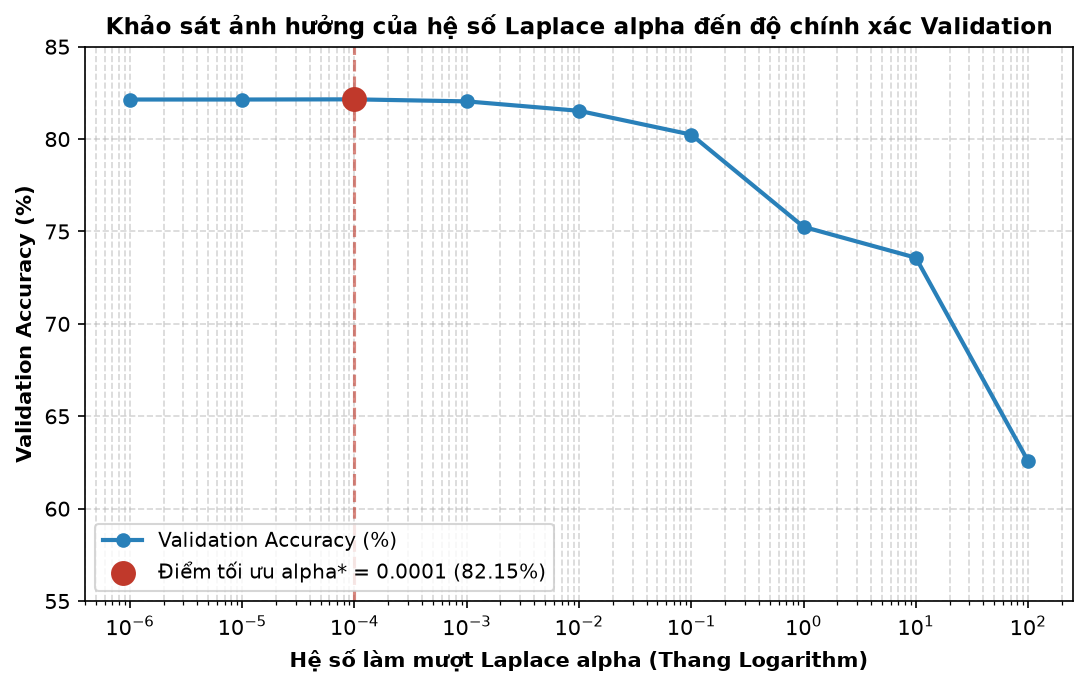
\includegraphics[height=2.8cm, keepaspectratio]{figures/1_01_laplace_alpha_tuning.png}
        \caption{Tinh chỉnh Laplace $\alpha$}
        \label{fig:1_01_alpha}
    \end{subfigure}
    \hfill
    \begin{subfigure}[b]{0.32\textwidth}
        \centering
        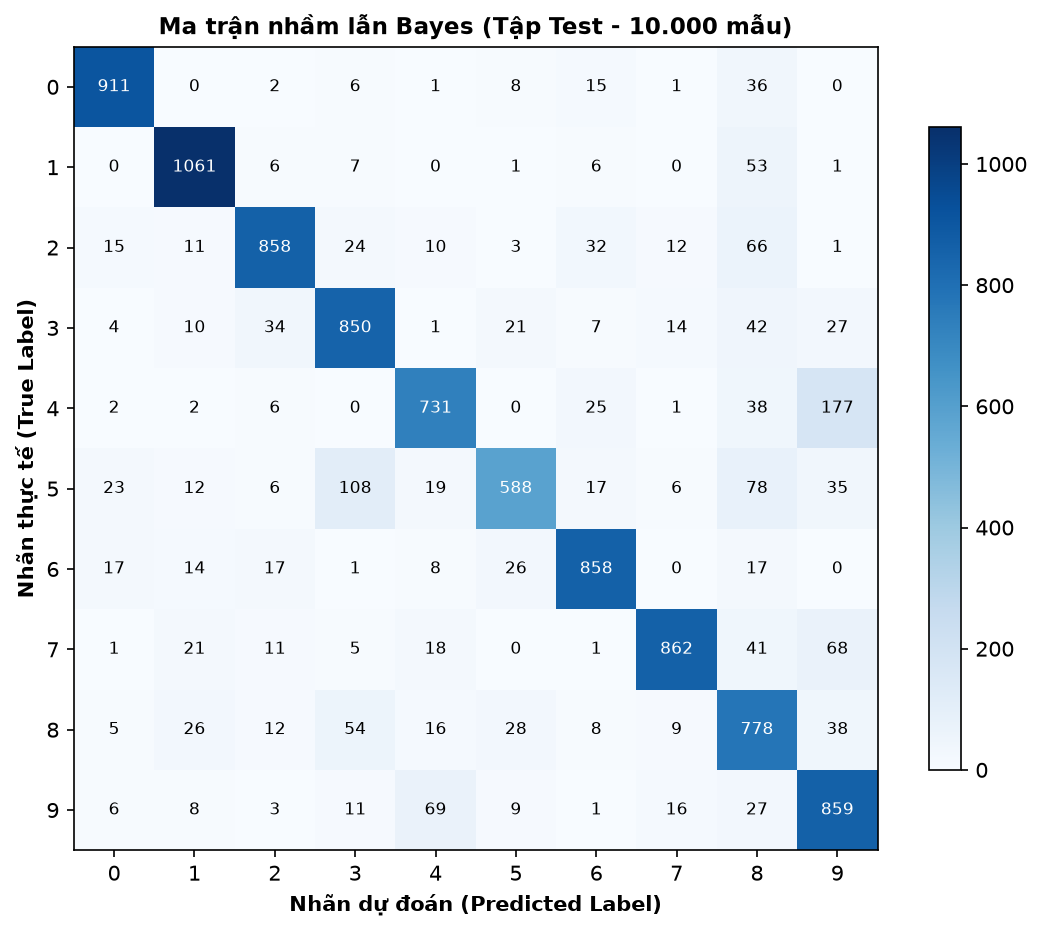
\includegraphics[height=2.8cm, keepaspectratio]{figures/1_04_bayes_confusion_test.png}
        \caption{Ma trận nhầm lẫn Naïve Bayes}
        \label{fig:1_04_bayes_cm}
    \end{subfigure}
    \hfill
    \begin{subfigure}[b]{0.32\textwidth}
        \centering
        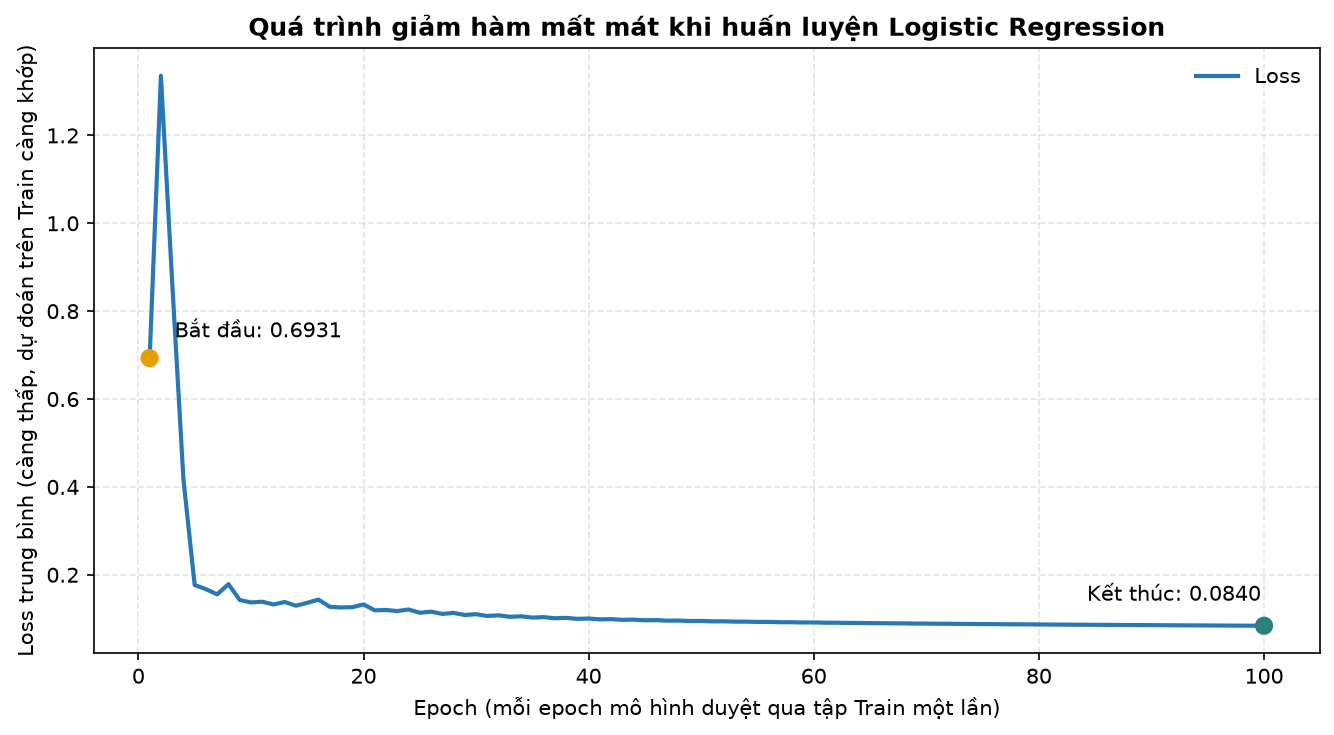
\includegraphics[height=2.8cm, keepaspectratio]{figures/2_02_logistic_loss_curve.png}
        \caption{Đường cong mất mát Logistic}
        \label{fig:2_02_loss}
    \end{subfigure}
    
    \vspace{0.15cm}
    \begin{subfigure}[b]{0.48\textwidth}
        \centering
        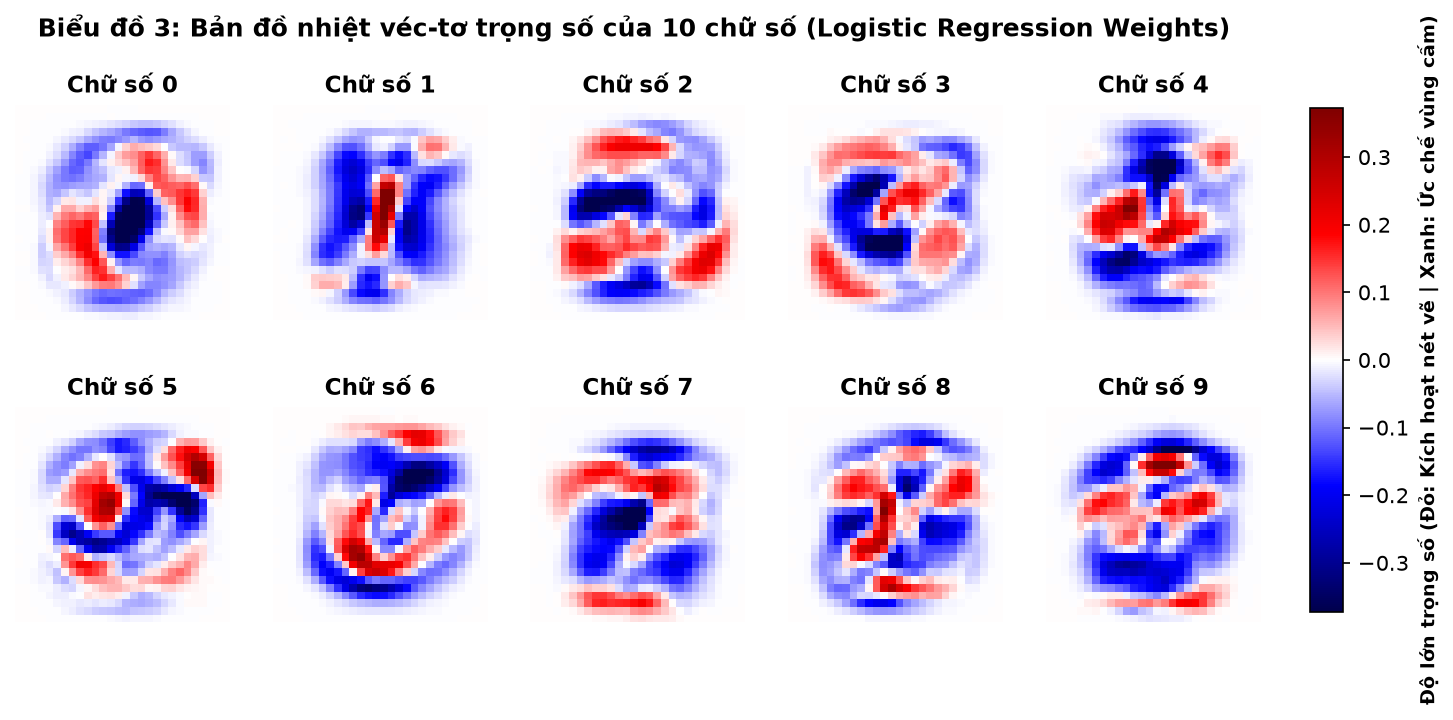
\includegraphics[height=2.8cm, keepaspectratio]{figures/2_03_logistic_weights.png}
        \caption{Trực quan hóa ma trận trọng số $W$}
        \label{fig:2_03_weights}
    \end{subfigure}
    \hfill
    \begin{subfigure}[b]{0.48\textwidth}
        \centering
        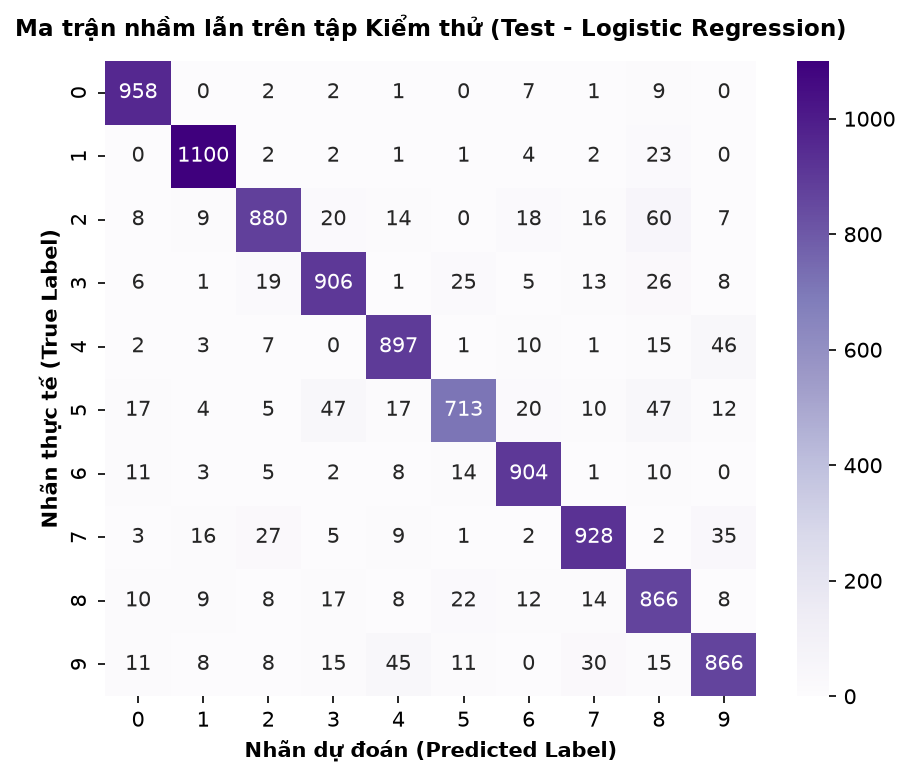
\includegraphics[height=2.8cm, keepaspectratio]{figures/2_06_logistic_confusion_test.png}
        \caption{Ma trận nhầm lẫn Logistic Test}
        \label{fig:2_06_logistic_cm}
    \end{subfigure}
    \caption{Kết quả thực nghiệm mô hình Naïve Bayes và Hồi quy Logistic From-Scratch}
    \label{fig:scratch_models_perf}
\end{figure}

\subsubsection{Mô hình Học sâu (\code{3\_MLP\_CNN}) và Học kết hợp (\code{4\_Ensemble})}
Khảo sát động học học sâu chứng minh: ReLU duy trì chuẩn gradient ổn định ($0.15 - 0.20$), khắc phục hiện tượng suy giảm gradient theo cấp số nhân của Sigmoid (Hình~\ref{fig:3_03_grad}); phép khởi tạo He bảo toàn độ lệch chuẩn đầu ra kích hoạt qua các tầng ($0.6 - 0.8$), ngăn ngừa triệt tiêu tín hiệu như khởi tạo hằng số (Hình~\ref{fig:3_04_var}).

Về hiệu năng, \code{MLP} đạt độ chính xác \textbf{98.26\%} (chỉ nhầm 174/10.000 mẫu) sau 18 epoch huấn luyện trong $38.36$s (Hình~\ref{fig:3_01_mlp_hist}). \code{CNN} dẫn đầu tuyệt đối với \textbf{98.76\%} (chỉ nhầm 124 mẫu trên toàn bộ $10.000$ mẫu test, Hình~\ref{fig:3_07_cnn_cm}). Đối với nhóm Boosting (Hình~\ref{fig:4_01_ens_acc}), \code{AdaBoost (depth=3)} đạt $91.75\%$ nhờ khả năng học tương tác phi tuyến cục bộ của cây quyết định (Hình~\ref{fig:4_03_feat}); trong khi \code{AdaBoost (LogReg)} đạt $85.06\%$, \code{AdaBoost (stump)} đạt $78.53\%$, và \code{AdaBoost (GaussianNB)} suy thoái xuống $56.41\%$.

\begin{figure}[htbp]
    \centering
    \begin{subfigure}[b]{0.32\textwidth}
        \centering
        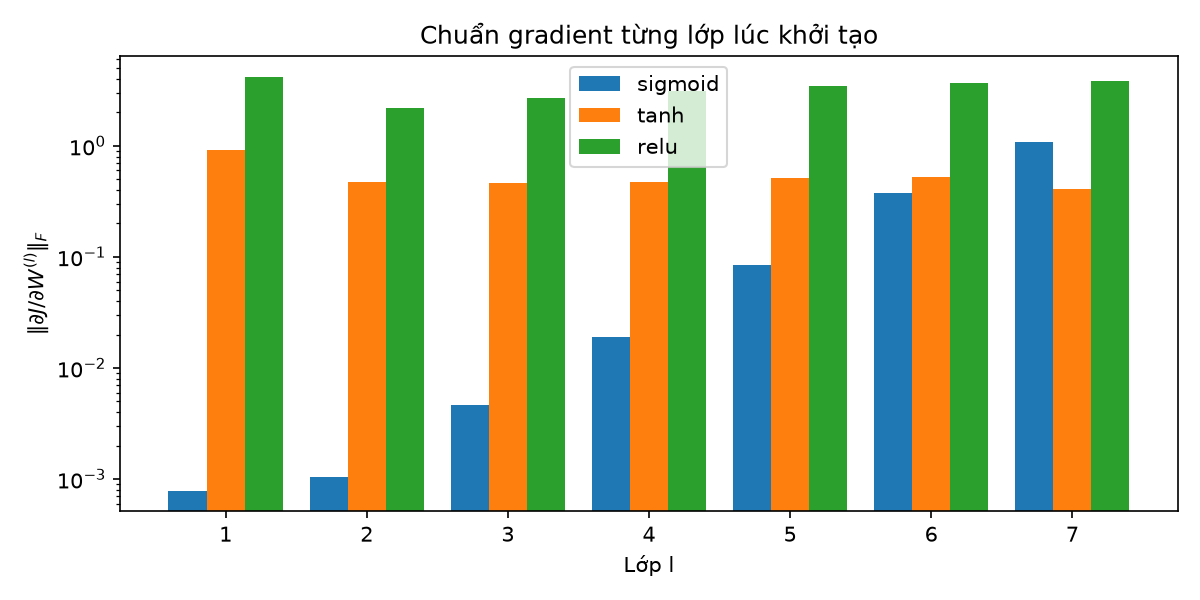
\includegraphics[height=2.8cm, keepaspectratio]{figures/3_03_vanishing_gradient.png}
        \caption{Gradient qua các tầng}
        \label{fig:3_03_grad}
    \end{subfigure}
    \hfill
    \begin{subfigure}[b]{0.32\textwidth}
        \centering
        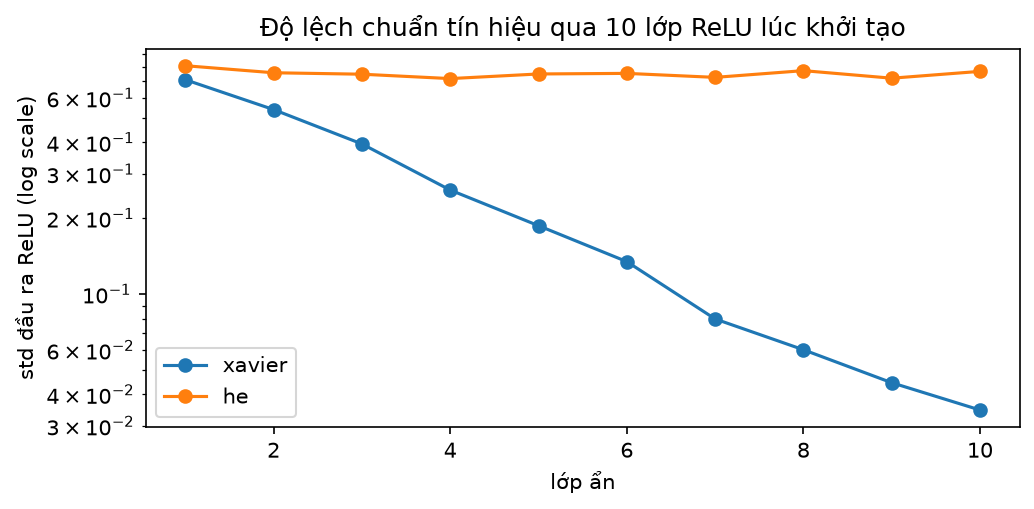
\includegraphics[height=2.8cm, keepaspectratio]{figures/3_04_variance_preservation.png}
        \caption{Bảo toàn phương sai He}
        \label{fig:3_04_var}
    \end{subfigure}
    \hfill
    \begin{subfigure}[b]{0.32\textwidth}
        \centering
        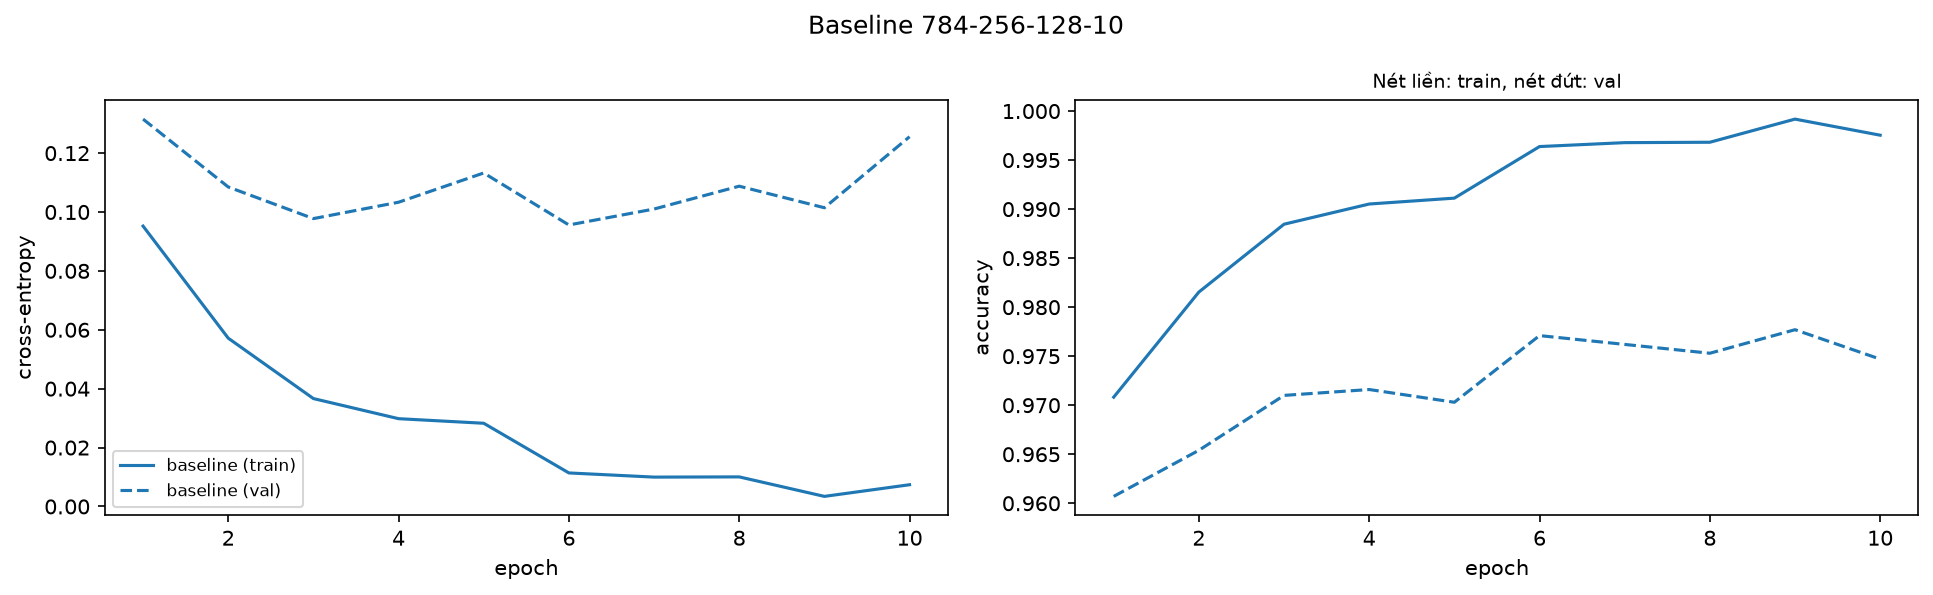
\includegraphics[height=2.8cm, keepaspectratio]{figures/3_01_baseline_mlp_history.png}
        \caption{Lịch sử huấn luyện MLP}
        \label{fig:3_01_mlp_hist}
    \end{subfigure}

    \vspace{0.15cm}
    \begin{subfigure}[b]{0.32\textwidth}
        \centering
        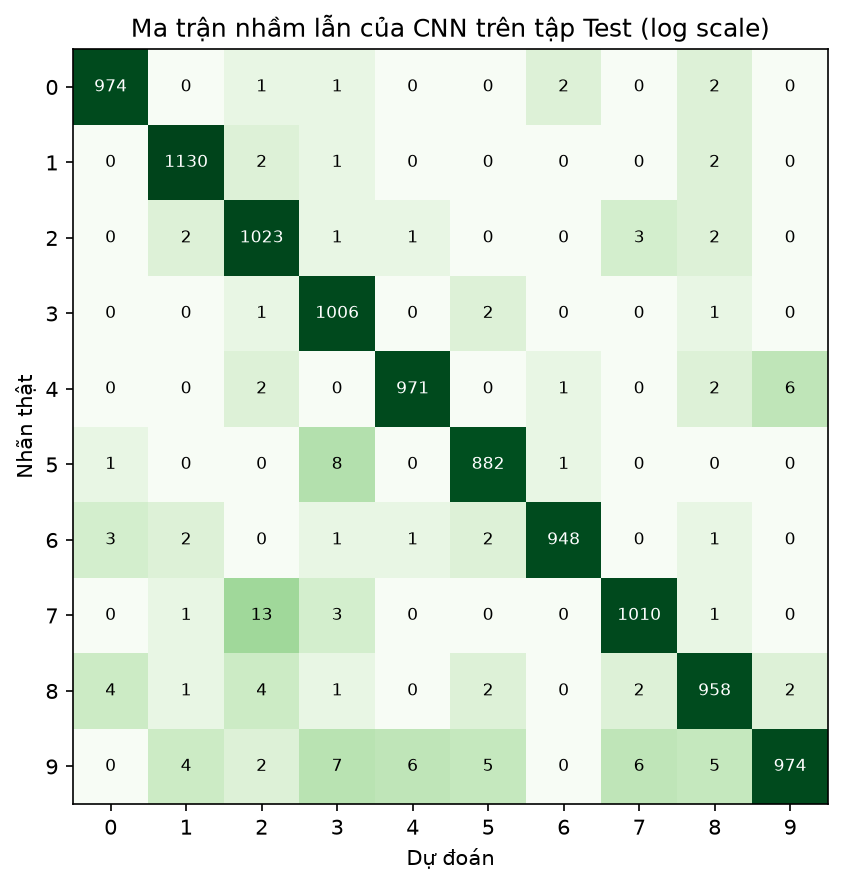
\includegraphics[height=2.8cm, keepaspectratio]{figures/3_07_cnn_confusion_matrix.png}
        \caption{Ma trận nhầm lẫn CNN}
        \label{fig:3_07_cnn_cm}
    \end{subfigure}
    \hfill
    \begin{subfigure}[b]{0.32\textwidth}
        \centering
        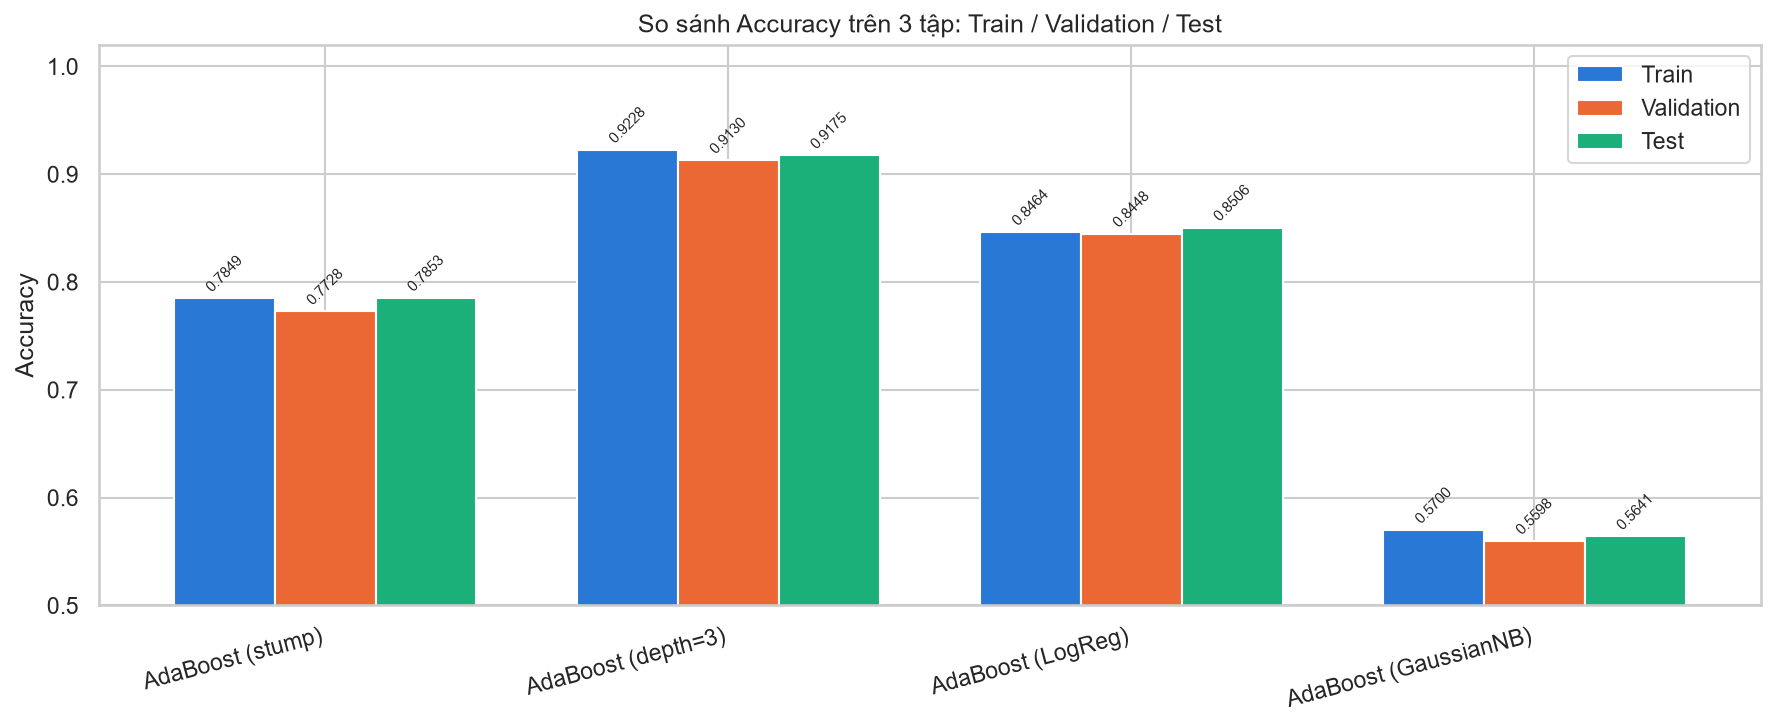
\includegraphics[height=2.8cm, keepaspectratio]{figures/4_01_accuracy_comparison.png}
        \caption{Độ chính xác AdaBoost}
        \label{fig:4_01_ens_acc}
    \end{subfigure}
    \hfill
    \begin{subfigure}[b]{0.32\textwidth}
        \centering
        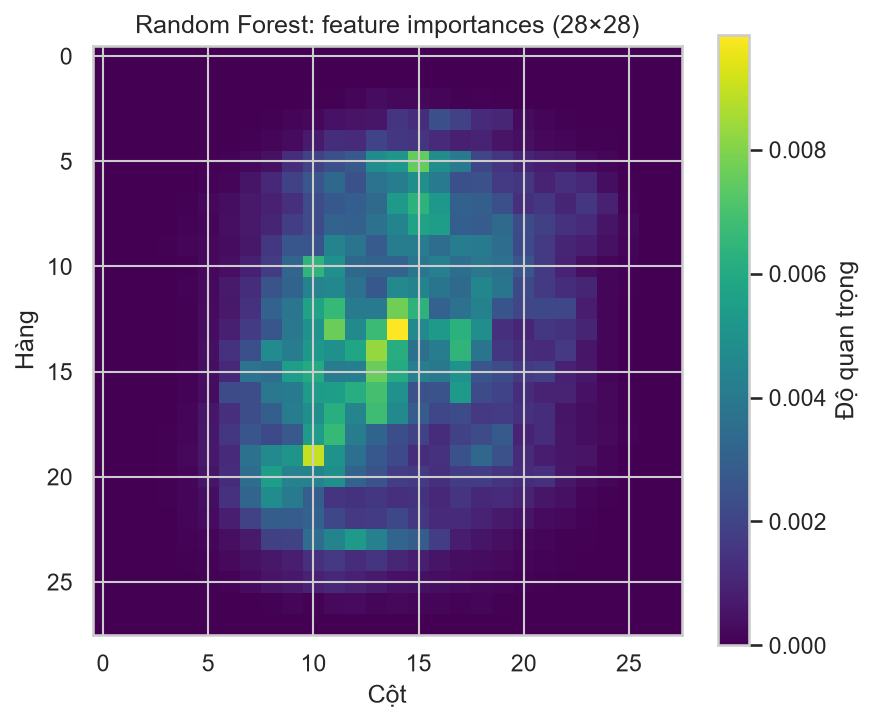
\includegraphics[height=2.8cm, keepaspectratio]{figures/4_03_feature_importances.png}
        \caption{Tầm quan trọng pixel AdaBoost}
        \label{fig:4_03_feat}
    \end{subfigure}
    \caption{Kết quả thực nghiệm mạng Học sâu (MLP, CNN) và Học kết hợp Boosting}
    \label{fig:dl_ensemble_perf}
\end{figure}

\subsection{Bảng tổng hợp so sánh chung trên tập Test}
Bảng~\ref{tab:overall_comparison} tổng hợp toàn bộ các thước đo hiệu năng trên tập kiểm thử độc lập ($10.000$ mẫu ảnh), được trích xuất trực tiếp từ tệp \code{results/overall\_comparison\_metrics.csv}.

\begin{table}[htbp]
    \centering
    \footnotesize
    \caption{Bảng tổng hợp đối chiếu hiệu năng các mô hình trên tập Test ($10.000$ mẫu)}
    \label{tab:overall_comparison}
    \vspace{0.15cm}
    \renewcommand{\arraystretch}{1.15}
    \begin{tabular}{llrrrrrrr}
        \toprule
        \textbf{Nguồn} & \textbf{Mô hình} & \textbf{Acc (\%)} & \textbf{Macro-F1} & \textbf{Prec (\%)} & \textbf{Rec (\%)} & \textbf{Train (s)} & \textbf{Test (s)} & \textbf{Độ trễ} \\
        \midrule
        \code{1\_Bayes} & MultinomialNB-NP & 83.56 & 83.41\% & 84.24 & 83.25 & \textbf{0.06} & 0.3330 & 33.30 $\mu\text{s}$ \\
        \code{2\_Logistic} & LogisticRegression-NP & 90.18 & 90.03\% & 90.17 & 90.03 & 32.29 & 0.0259 & 2.59 $\mu\text{s}$ \\
        \code{3\_MLP\_CNN} & MLP & 98.26 & 98.25\% & 98.25 & 98.24 & 38.36 & \textbf{0.0246} & \textbf{2.46 $\mu\text{s}$} \\
        \code{3\_MLP\_CNN} & CNN & \textbf{98.76} & \textbf{98.76\%} & \textbf{98.77} & \textbf{98.75} & 56.90 & 0.5319 & 53.19 $\mu\text{s}$ \\
        \midrule
        \code{4\_Ensemble} & AdaBoost (depth=3) & 91.75 & 91.70\% & 91.81 & 91.70 & 11019.24 & 2.6681 & 266.81 $\mu\text{s}$ \\
        \code{4\_Ensemble} & AdaBoost (LogReg) & 85.06 & 84.85\% & 85.11 & 84.79 & 48.39 & 0.3013 & 30.13 $\mu\text{s}$ \\
        \code{4\_Ensemble} & AdaBoost (stump) & 78.53 & 78.37\% & 78.80 & 78.26 & 241.97 & 2.4197 & 241.97 $\mu\text{s}$ \\
        \code{4\_Ensemble} & AdaBoost (GaussianNB) & 56.41 & 50.83\% & 71.58 & 55.63 & 46.76 & 7.8411 & 784.11 $\mu\text{s}$ \\
        \bottomrule
    \end{tabular}
\end{table}

\subsection{Trực quan hóa so sánh tổng thể}
\begin{figure}[htbp]
    \centering
    \begin{subfigure}[b]{0.32\textwidth}
        \centering
        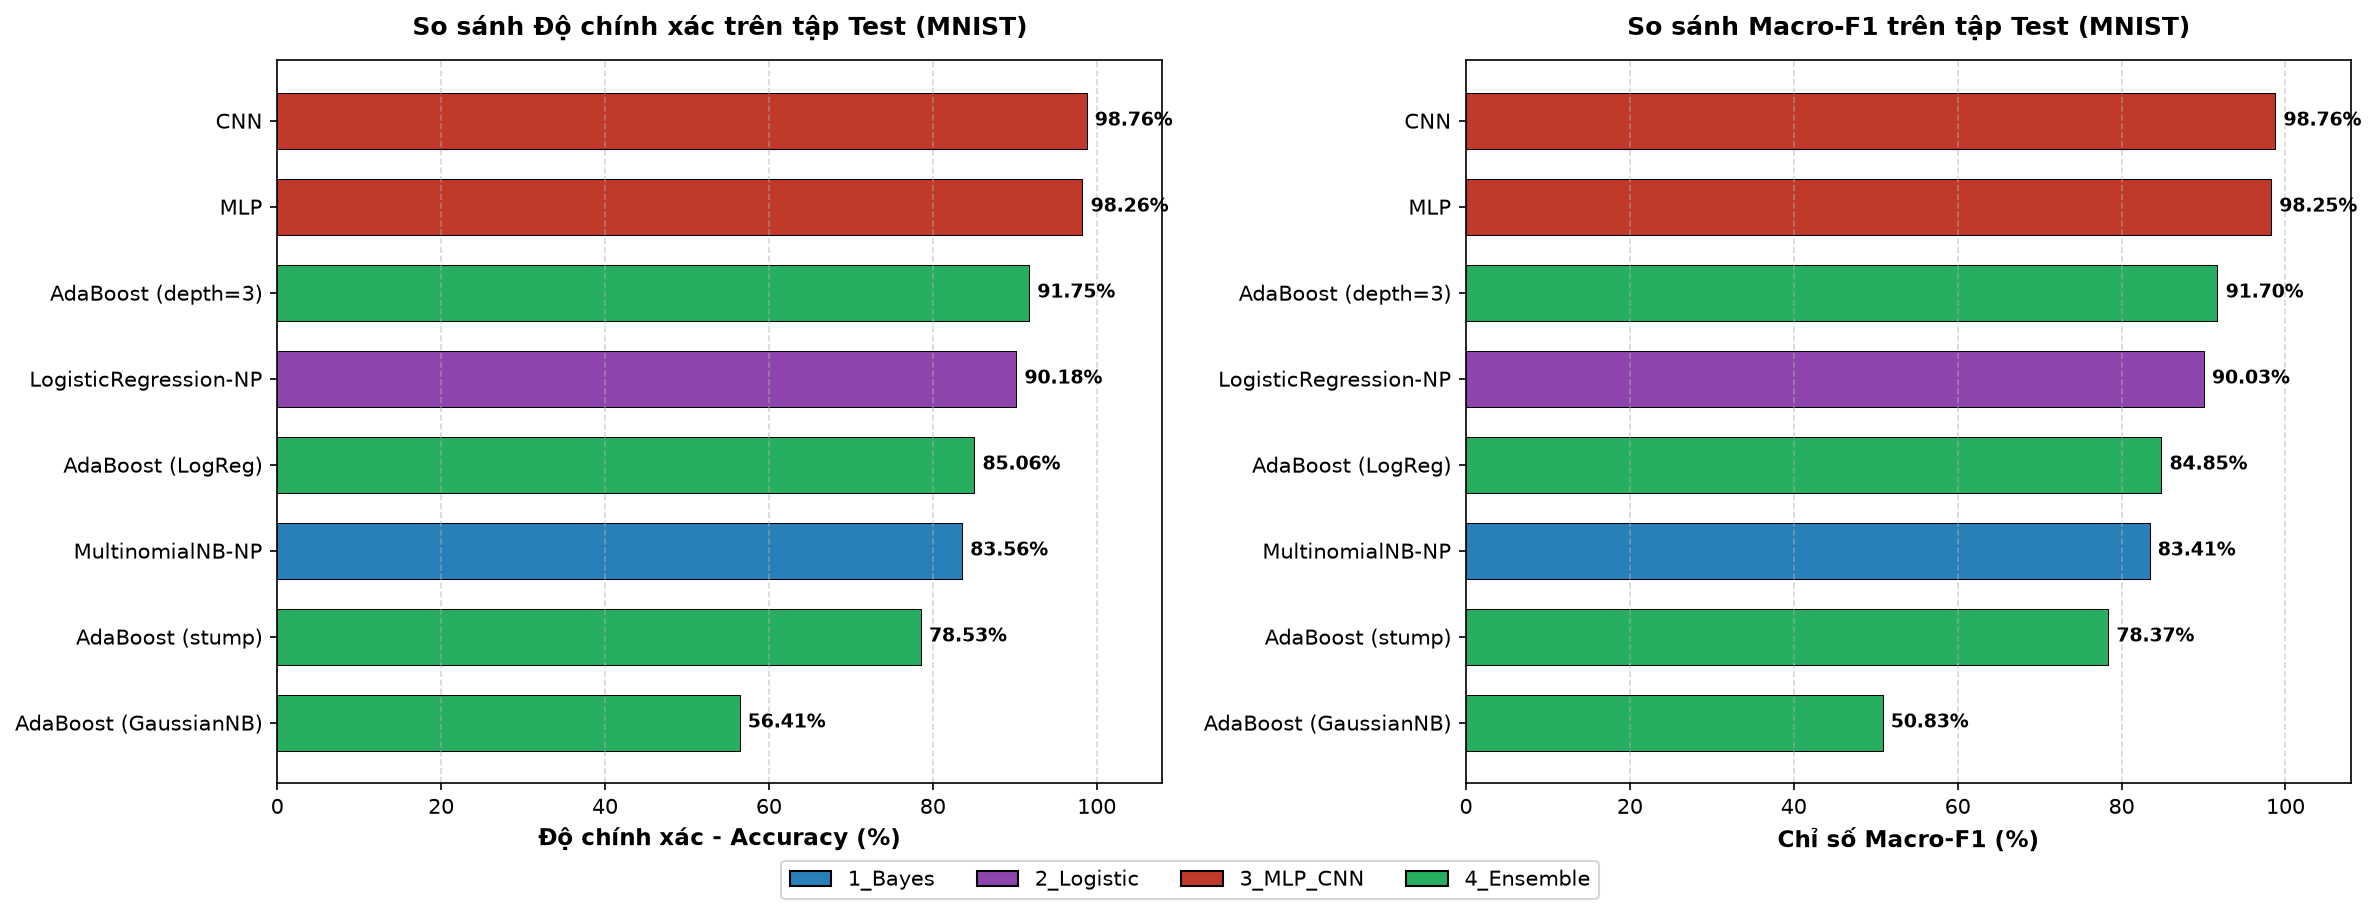
\includegraphics[height=3.3cm, keepaspectratio]{figures/Comp_01_accuracy_f1_comparison.png}
        \caption{Accuracy và Macro-F1}
        \label{fig:comp_01_acc_f1}
    \end{subfigure}
    \hfill
    \begin{subfigure}[b]{0.32\textwidth}
        \centering
        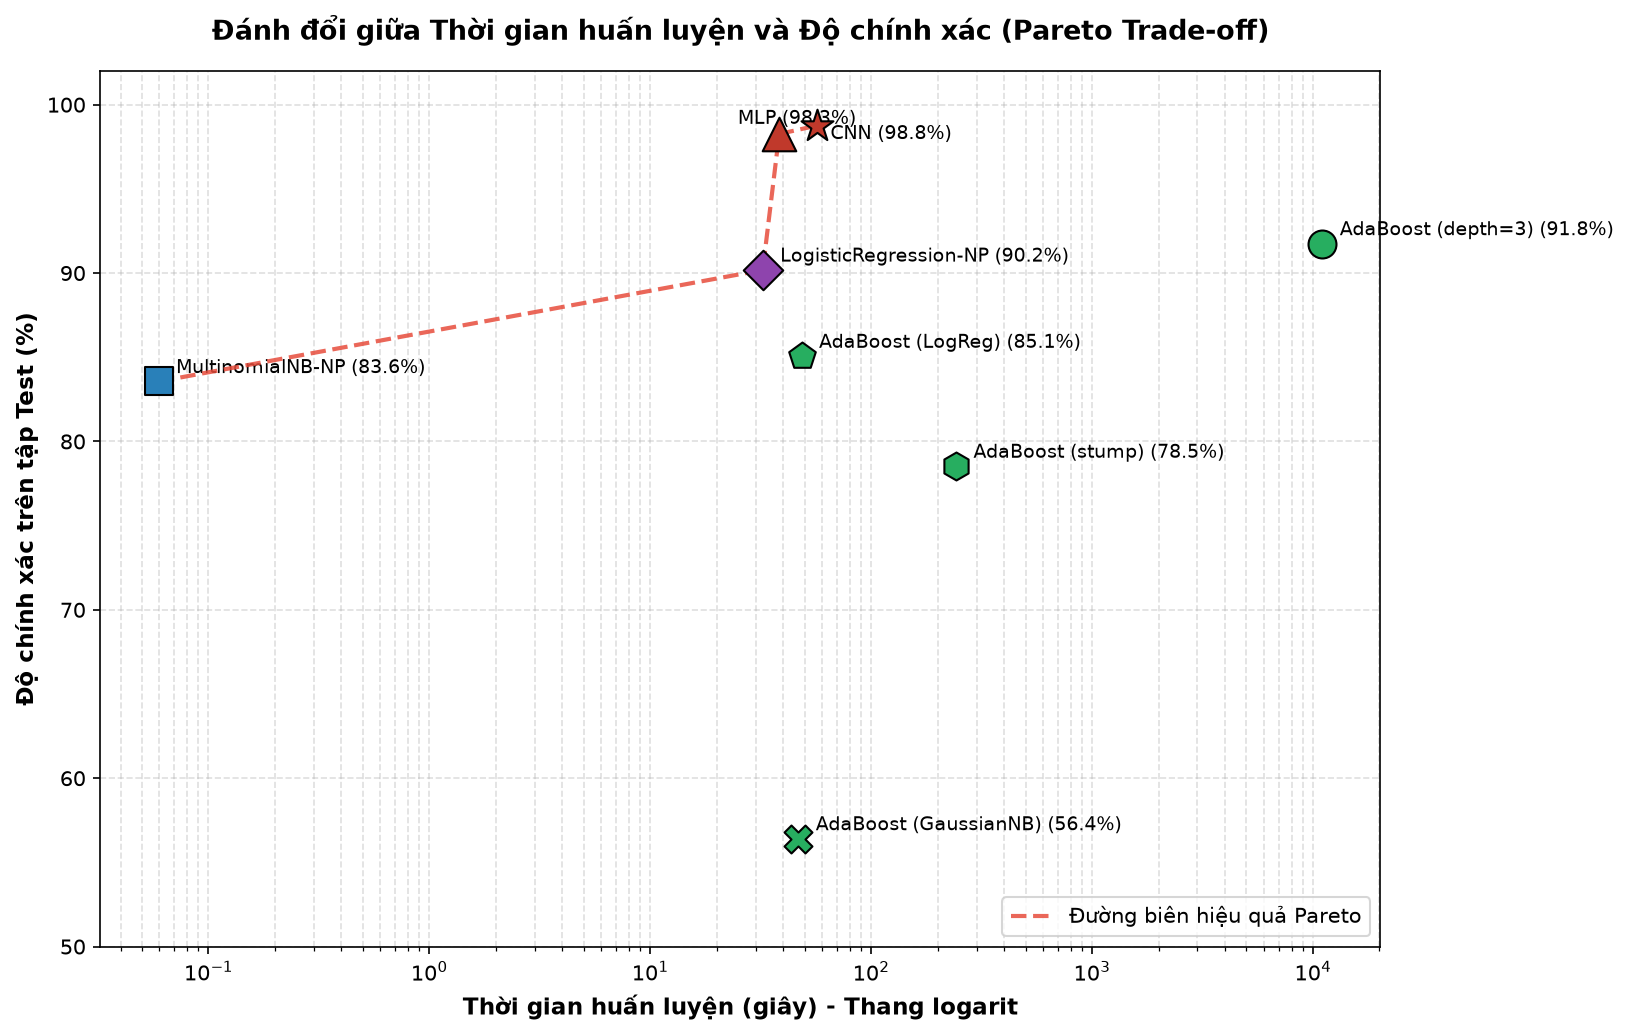
\includegraphics[height=3.3cm, keepaspectratio]{figures/Comp_02_time_vs_accuracy_pareto.png}
        \caption{Đánh đổi Train vs. Acc (Pareto)}
        \label{fig:comp_02_pareto}
    \end{subfigure}
    \hfill
    \begin{subfigure}[b]{0.32\textwidth}
        \centering
        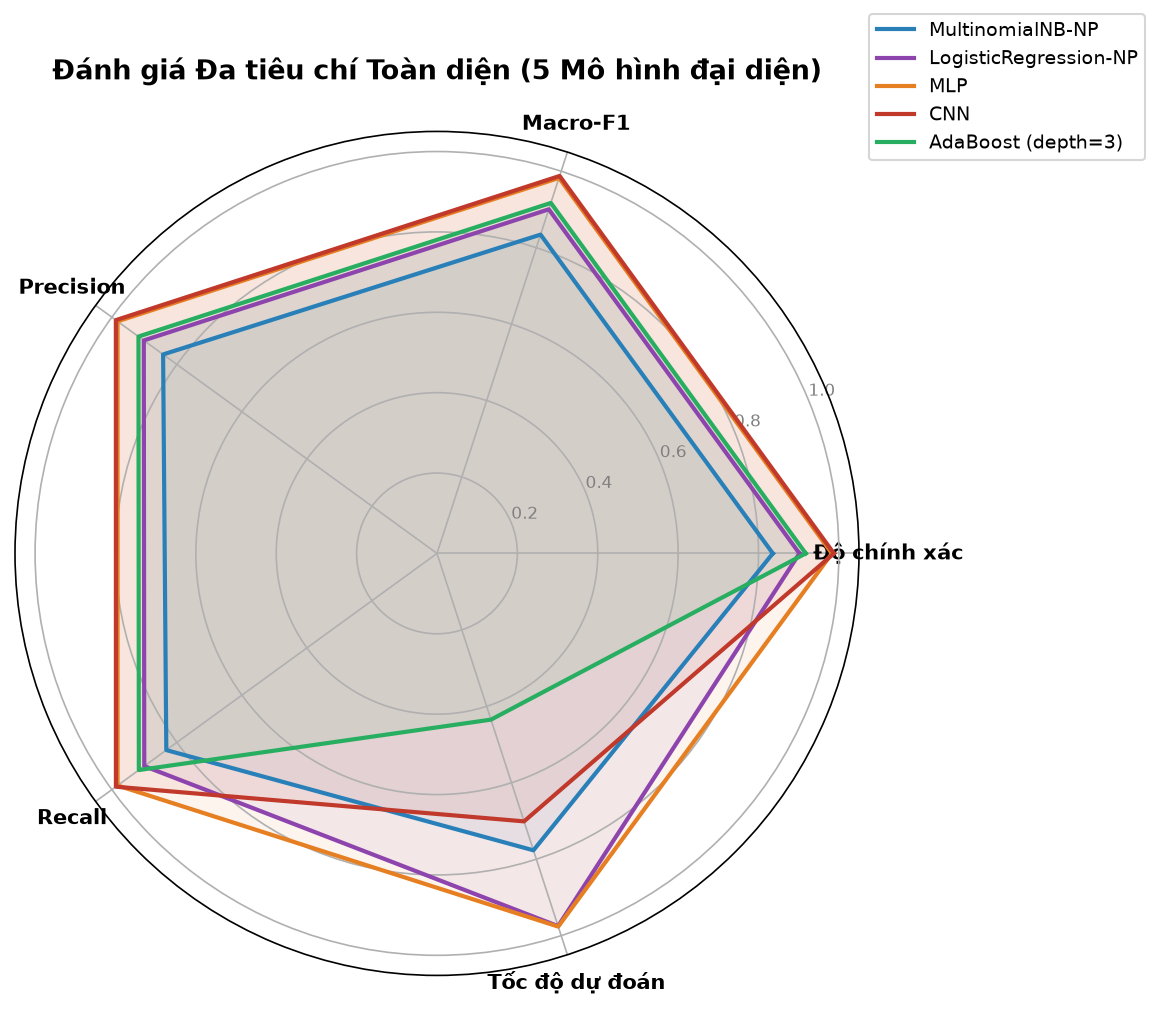
\includegraphics[height=3.3cm, keepaspectratio]{figures/Comp_03_radar_multi_criteria.png}
        \caption{Radar đa tiêu chí chuẩn hóa}
        \label{fig:comp_03_radar}
    \end{subfigure}
    \caption{Phân tích tương quan hiệu năng toàn diện, đường biên Pareto và biểu đồ Radar}
    \label{fig:comp_all_charts}
\end{figure}

Phân tích 3 biểu đồ tổng hợp:
\begin{enumerate}
    \item \textbf{Độ chính xác và Macro-F1 (Hình~\ref{fig:comp_01_acc_f1}):} Phổ điểm số phân tách thành 3 nhóm rõ rệt: nhóm xuất sắc gồm CNN ($98.76\%$) và MLP ($98.26\%$); nhóm khá gồm AdaBoost depth=3 ($91.75\%$) và Logistic ($90.18\%$); nhóm trung bình/kém gồm AdaBoost LogReg ($85.06\%$), Naïve Bayes ($83.56\%$), AdaBoost stump ($78.53\%$) và AdaBoost GaussianNB ($56.41\%$).
    \item \textbf{Đường biên hiệu quả Pareto (Hình~\ref{fig:comp_02_pareto}):} Định hình bởi ba mô hình then chốt: \code{MultinomialNB-NP} cực nhanh ($0.06$s, $83.56\%$); \code{MLP} đạt tỷ suất tối ưu nhất ($38.36$s, $98.26\%$); và \code{CNN} đạt đỉnh độ chính xác ($56.90$s, $98.76\%$). Ngược lại, \code{AdaBoost (depth=3)} nằm rất xa đường biên Pareto khi tiêu tốn tới $11.019$s nhưng độ chính xác thua kém các mạng nơ-ron $6.5\% - 7.0\%$.
    \item \textbf{Biểu đồ Radar đa tiêu chí (Hình~\ref{fig:comp_03_radar}):} \code{MLP} có diện tích bao phủ rộng và cân đối nhất nhờ sự kết hợp đồng thời giữa độ chính xác cao, thời gian huấn luyện ngắn và độ trễ suy diễn nhanh nhất.
\end{enumerate}
